
\documentclass[12pt]{extarticle}
\oddsidemargin=-0.5in
\textwidth=7.0in
\topmargin=-.75in
\textheight=9.4in
\parskip=3mm
\parindent=0mm
\usepackage{graphicx}
%\usepackage{epsf}
%\usepackage{url}
\usepackage{hyperref}


\begin{document}
\pagestyle{empty}
\begin{center}
  {\Large {\bf Homework 09}}\\
%\medskip
%  {\large {\bf Cumulative Distributions}}\\
\medskip
{\large {\bf Calculus II}}\\
\medskip
{\bf College of the Atlantic. Due March 14, 2025}\\
\end{center}

\medskip

There is also a WeBWorK assignment. It is only one problem. 

It is well known that the average mass of wild unicorns is 100 kg with 
a standard deviation of 12. 

\begin{enumerate}
\setlength{\itemsep}{3mm}
\item In your cosmic ray unicorn-creation
experiments you have created 55 unicorns. You measure the masses of
these 55 unicorns and determine that their average mass is 96. 
Hmmm... Is the mass of this group of unicorns unusually low compared
to wild unicorns? 
\begin{enumerate}
%  \setlength{\itemsep}{15mm}
  \item If you sampled 55 wild unicorns, how would that mean be
    distributed?
  \item How likely is it that if you sampled 55 wild unicorns you
    would get a mean of 96 or smaller. Write the answer as an
    integral, and then use a computer to evaluate the integral. (You
    just calculated a one-tailed p-value. Congratulations.)
  \item How likely is it that if you sampled 55 wild unicorns you
        would get a mean that was smaller than 96 or larger than
        104. Write the answer as an integral, and then determine a
        numerical value for the intergral.  (You just calculated a
        two-tailed p-value. Congratulations, again.)
\end{enumerate}


\item Repeat the above question for an experimental run in which you
  generated 55 unicorns and their average mass is 99 kg.
  
\item Repeat the above question for an experimental run in which you
  generated 900 unicorns and their average mass is 99 kg.

\end{enumerate}


\begin{figure}[b!]
\begin{center}
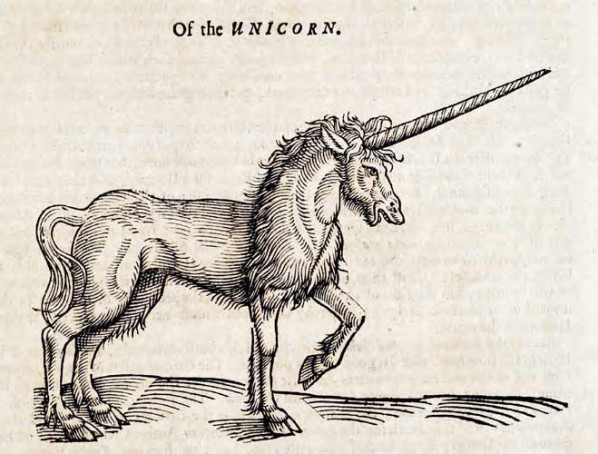
\includegraphics[width=3.0in]{Oftheunicorn.jpg}
\vspace{1mm}
\caption{An illustration from the book The history of four-footed
  beasts and serpents by Edward Topsell. Special Collections,
  University of Huston Libraries. Creative Commons CC0 1.0 Universal
  Public Domain Dedication. \href{https://commons.wikimedia.org/wiki/File:Oftheunicorn.jpg}{https://commons.wikimedia.org/wiki/File:Oftheunicorn.jpg}.}
%\caption{A unicorn. Image from \protect\url{
%    https://freesvg.org/unicorn-for-coloring}}
%\label{fig:speed}
\end{center}
\end{figure}


\end{document}



